\documentclass[class=report, crop=false, 12pt,a4paper]{standalone}
\usepackage{graphicx}
\usepackage{float}
\usepackage{amsmath}
\usepackage{amssymb}
\usepackage{siunitx}
\usepackage{commath}
\usepackage[a4paper,width=150mm,top=25mm,bottom=25mm]{geometry}
\begin{document}
\section{Reynold's number}
Reynolds conducted experiments, in which he measured pressure drop and critical velocity in a variety of pipe diameters and with different fluids, and verified the importance of the parameter $\frac{\rho d \vec{U}}{\mu}$ later to be given his name. He found that, instead of a different critical velocity for each fluid and pipe, the onset of turbulence (i.e. transition) was determined by the achievement of the same critical value of Reynolds number, usually quoted as:
\begin{equation}
  Re_{d,crit} = 2300
\end{equation}
We note the confirmation of the empirical results regarding critical velocity because if:
\begin{equation}
  Re_{d,crit} = \frac{\rho d \vec{U}_{crit}}{\mu} = 2300
\end{equation}
then $\vec{U} \propto \frac{1}{d}$ for given $\rho$ and $\mu$ and $\vec{U}_{crit} \propto \mu$ for given $d$ and $\mu$.
\begin{figure}[H]
  \centering
  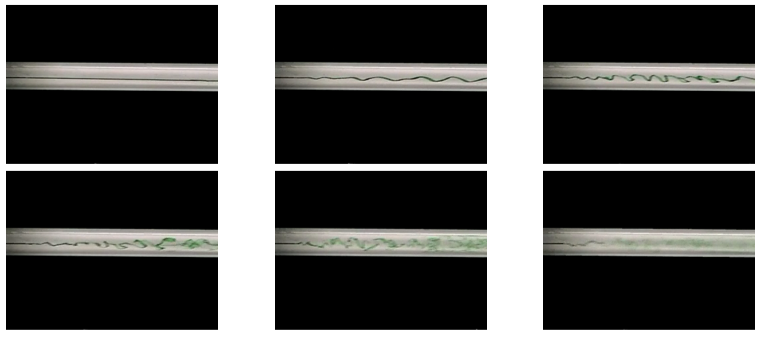
\includegraphics[width = 0.9 \textwidth]{../img/diagram78.png}
  \caption{}
\end{figure}
\begin{itemize}
  \item In this experiment water flows through a clear pipe with increasing speed
  \item Dye is injected through a small diameter tube at the left portion of the screen
  \item At low speed $ \left( Re < 2300 \right)$ the flow is laminar and the dye is a straight line
  \item As the speed increases, the dye stream becomes wavy (oscillatory laminar flow)
  \item At still higher speeds $\left(Re > 4000\right)$ the flow becomes turbulent and the dye stream is dispersed randomly throughout the flow
\end{itemize}
\section{Flow in pipes}
\subsection{Entrance region}
\begin{figure}[H]
  \centering
  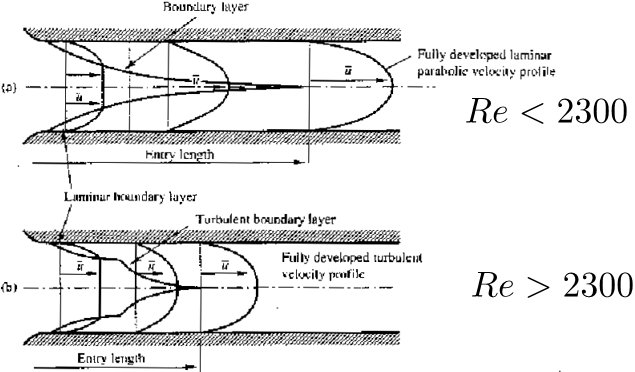
\includegraphics[width = 0.9 \textwidth]{../img/diagram79.png}
  \caption{}
\end{figure}
Reynolds number: $Re = \frac{\rho \vec{U} D}{\mu}$ where $D$ is the diameter.
\begin{figure}[H]
  \centering
  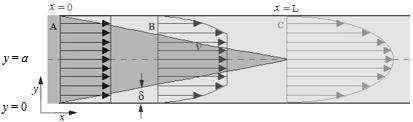
\includegraphics[width = 0.6 \textwidth]{../img/diagram80.png}
  \caption{}
\end{figure}
\begin{itemize}
  \item The nature of the flow in the entrance region and hence its length, depend on whether the fully-developed flow is laminar or turbulent
  \begin{itemize}
    \item \makebox[4cm]{$Re_d < 2300$:\hfill} Fully-developed flow should be laminar
    \item \makebox[4cm]{$Re_d > 2300$:\hfill} Fully-developed flow should be turbulent
    \item \makebox[4cm]{$2000 < Re_d < 3000$:\hfill} Transitional flow...
  \end{itemize}
  \item Figures given for laminar entry length variety
  \begin{itemize}
    \item \makebox[3cm]{\textit{Laghaar} quotes:\hfill} Entry length $=0.057 d Re_d$
    \item \makebox[3cm]{Rule of thumb:\hfill} Entry length $=100d$ minimum
  \end{itemize}
  \item For turbulent flow the fully-developed state is achieved much sooner (entry length less dependent on $Re_d$)
  \begin{itemize}
    \item \makebox[3cm]{Rule of thumb:\hfill} Entry length $=50d$ minimum
  \end{itemize}
\end{itemize}
\subsection{Shear stress}
What is the shear stress distribution in fully-developed pipe flows? Consider an axial cylindrical element of length $L$ within a pipe.
\begin{figure}[H]
  \centering
  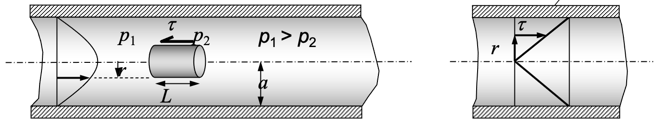
\includegraphics[width = 0.9 \textwidth]{../img/diagram81.png}
  \caption{}
\end{figure}
The forces due to pressure and shear (from velocity gradient) must balance out:
\begin{equation}
  p_1 \pi r^2 - p_2 \pi r^2 - \tau 2 \pi r L = 0 \rightarrow \tau = \frac{p_1 - p_2}{L} \frac{r}{2} = \frac{\Delta p}{L} \frac{r}{2} 
\end{equation}
This relationship is valid for both laminar and turbulent motion and shows that shear stress must vary linearly with radius $r$ in the pipe. The value of $\tau$ at the wall $\left( r = a \right)$ is: $\tau_w = \frac{\Delta p}{L} \frac{a}{2}$ so that: $\frac{\tau}{\tau_w} = \frac{r}{a}$. Wall shear stress can be measured by the pressure gradient in the pipe.
\section{Laminar flow in pipes}
\subsection{Velocity profile}
Laminar motion $\left(Re < 2300\right)$. What is the velocity profile? If the motion is laminar, the shear stress is easily related to the velocity gradient through the dynamic viscosity, $\mu$.
\begin{figure}[H]
  \centering
  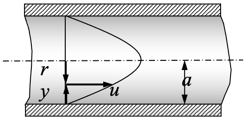
\includegraphics[width = 0.3 \textwidth]{../img/diagram82.png}
  \caption{}
\end{figure}
\begin{equation}
  \tau = \mu \frac{\dif u}{\dif y} \textrm{ where } y = a-r \textrm{ such that: } \dif y = -\dif r
\end{equation}
\begin{itemize}
  \item From previous result: $\tau = - \mu \frac{\dif u}{\dif r} = \frac{\Delta p}{L} \frac{r}{2}$
  \item Thus: $\dif u = - \frac{\Delta p}{2L} \frac{r}{\mu} \dif r$ which we can integrate to get: $u = - \frac{\Delta p}{4L\mu} r^2 + C$
  \item No slip boundary condition says: $u = 0$ at $ r = a \rightarrow C = \frac{\Delta p}{4 L \mu} a^2$
  \item Thus, finally: $u = \frac{1}{4\mu} \frac{\Delta p}{L} \left(a^2 - r^2\right)$ Parabolic velocity profile (\textit{Hagen-Poiseuille Law})
\end{itemize}
Segment V6.6 Laminar flow (Related to textbook section 6.9.3 - Steady, Laminar flow in circular tubes) The velocity distribution is parabolic for steady, laminar flow in circular tubes. A filament of dye is placed across a circular tube containing a very viscous liquid which is initially at rest. With the opening of a valve at the bottom of the tube the liquid starts to flow, and the parabolic velocity distribution is revealed. Although the flow is actually unsteady, it is quasi-steady since it is only slowly changing. Thus, at any instant in time the velocity distribution corresponds to the characteristic steady-flow parabolic distribution.
\subsection{Flow rate}
\begin{figure}[H]
  \centering
  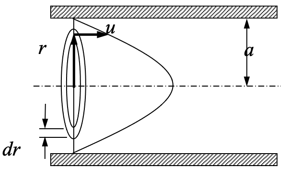
\includegraphics[width = 0.3 \textwidth]{../img/diagram83.png}
  \caption{}
\end{figure}
Parabolic velocity profile:
\begin{equation}
  u = \frac{1}{4\mu} \frac{\Delta p}{L} \left( a^2 - r^2\right)
\end{equation}
The maximum velocity $U_{max}$ occurs on the centre-line of the pipe (i.e. at $r=0$):
\begin{gather}
  U_{max} = \frac{1}{4\mu} \frac{\Delta p}{L}a^2\\
  \frac{u}{U_{max}} = \frac{a^2 - r^2}{a^2} \rightarrow \frac{u}{U_{max}} = 1 - \frac{r^2}{a^2}
\end{gather}
The mean velocity/flow rate is given by:
\begin{align}
  \vec{U} &= \frac{Q}{A} = \frac{\int_{0}^{a} \left(2\pi r u \right) \,\textrm{d}r}{\pi a^2}\\
  \vec{U} &= \frac{2\pi}{\pi a^2} \int_{0}^{a} \left(r u \right) \,\textrm{d}r = \frac{2}{a^2} \int_{0}^{a} \left(U_{\max} \left(1 - \frac{r^2}{a^2}\right)r\right) \,\textrm{d}r \\
  \vec{U} &= \frac{2U_{max}}{a^2} \int_{0}^{a} \left(r-\frac{r^3}{a^2}\right) \,\textrm{d}r\\
  \vec{U} &= \frac{2U_{max}}{a^2} \left[ \frac{r^2}{2} - \frac{r^4}{4a^2} \right]_0^a = \frac{2U_{max}}{a^2} \left[ \frac{a^2}{2} - \frac{a^4}{4a^2} \right] = \frac{U_{max}}{2} 
\end{align}
For a parabolic profile the mean velocity is hald the maximum velocity:
\begin{equation}
  u = \frac{1}{4\mu} \frac{\Delta p}{L} \left(a^2 - r^2\right) \makebox[1cm]{} U_{max} = \frac{1}{4\mu} \frac{\Delta p }{L} a^2 \makebox[1cm]{} \vec{U} = \frac{1}{8\mu}\frac{\Delta p}{L} a^2
\end{equation}
The volumetric flow rate is: 
\begin{equation}
  Q = \pi a^2 \vec{U} = \frac{\pi}{8\mu}\frac{\Delta p}{L} a^4
\end{equation}
This can be used as a basis for measuring $\mu$ if all the other parameters can be measured sufficiently accurately.
\section{Friction factor (flow in pipes)}
We have seen that the pressure loss in a pipe (whether laminar or turbulent) is related to the wall shear stress by:
\begin{equation}
  \tau_w = \frac{\Delta p}{L}\frac{a}{2}
\end{equation}
A dimensionless representation of the wall shear stress (and therefore the pressure gradient) is given by the defining a friction factor as the ratio of wall shear stress to dynamic pressure in the flow (based on mean velocity).
\begin{equation}
  f = \frac{\tau_w}{\frac{1}{2}\rho \vec{U}^2}
\end{equation}
\subsection{Pressure drop due to friction}
Generalised expression for pressure drop due to friction. We have seen from equilibrium considerations (for laminar or turbulent flow) that: 
\begin{equation}
  \tau_w = \frac{\Delta p}{L} \frac{a}{2} = \frac{\delta p}{L} \frac{d}{4}
\end{equation}
Thus,
\begin{equation}
  \Delta p = \frac{4L\tau_w}{d}\rightarrow \Delta p =\frac{4L}{d} f \frac{1}{2} \rho \vec{U}^2
\end{equation}
Hence:
\begin{equation}
  h_f = \frac{\Delta p}{\rho g} \rightarrow h_f = \frac{4L}{d} f \frac{\vec{U}^2}{2g} \label{darcys}
\end{equation}
Eq.\ref{darcys} is known as \textit{Darcy's} Formula. To work out the pressure drop due to friction in pipe flows, we need to know accurately the friction factor $f$.
\section{Friction factor (laminar flow in pipes)}
Friction factor as a function of Reynolds number. Definition of friction factor (laminar or turbulent flow):
\begin{equation}
  f = \frac{\tau_w}{\frac{1}{2}\rho \vec{U}^2}
\end{equation}
For laminar flow we have:
\begin{equation}
  u = U_{max} \left(1-\frac{r^2}{a^2}\right) \makebox[1cm]{} \vec{U} = \frac{U_{max}}{2}
\end{equation}
Also:
\begin{gather}
  \tau_w = - \mu \left[\frac{\dif u}{\dif r}\right]_{r=a} = -\mu \left[\frac{-2\mu U_{max}a}{a^2}\right]_{r=a} = \frac{2\mu U_{max} a}{a^2} = \frac{2\mu U_{max}}{a} = \frac{4\mu U_{max}}{d}\\
  \tau_w = \frac{8\mu\vec{U}}{d}
\end{gather}
Thus, finally:
\begin{equation}
  f= \frac{\frac{8\mu\vec{U}}{d}}{\frac{1}{2}\rho \vec{U}^2} \rightarrow f = \frac{16\mu}{\rho d \vec{U}} \rightarrow f = \frac{16}{Re_d}
\end{equation}
\section{Laminar vs Turbulent profiles}
Segment V8.3 Laminar/Turbulent Velocity profiles (Related to textbook section 8.3.3 - Turbulent velocity profiles) The velocity profile for laminar flow in a pipe is quite different than that for turbulent flow. An approximation to the velocity profile in a a pipe is obtained by observing the motion of a dye streak placed across the pipe. With a viscous oil at Reynolds number of about 1, viscous effects dominate and it is easy to inject a relatively straight dye streak. The resulting laminar flow profile is parabolic. With water at Reynolds number of about 10000, inertial effects dominate and it is difficult to inject a straight dye streak. It is clear, however, that the turbulent velocity profile is not parabolic, but is more nearly uniform than for laminar flow.
\section{Turbulent flow in pipes}
\subsection{Velocity profile}
Due to chaotic nature of turbulence, turbulent flows are difficult to analyse and empirical relations mostly necessary. The time average velocity profile is much flatter than a laminar paraboloid:
\begin{figure}[H]
  \centering
  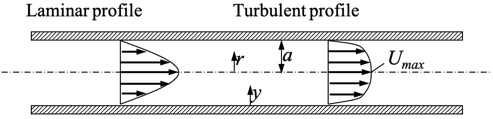
\includegraphics[width = 0.7 \textwidth]{../img/diagram84.png}
  \caption{}
\end{figure}
Approximate power laws used, depending on $Re_d$:
\begin{equation}
  \frac{u}{U_{max}} = \left( \frac{y}{a}\right)^{\frac{1}{n}} \textrm{ or } \frac{u}{U_{max}} = \left(\frac{a-r}{a}\right)^{\frac{1}{n}} \rightarrow \frac{u}{U_{max}} = \left(1-\frac{r}{a}\right)^{\frac{1}{n}}
\end{equation}
$n = 6-10$ but often taken as $n=7$, known as the \textit{"One-Seventh Power Law"}. It can be shown that the ratio of the mean velocity to the maximum velocity is:
\begin{align}
  \frac{\vec{U}}{U_{max}} = \frac{2n^2}{\left(n+1\right)\left(2n+1\right)}\approx 0.817 \textrm{ for }n=7
\end{align}
Also note that:
\begin{align}
  \frac{\dif u}{\dif y} = \frac{\dif}{\dif y}\left(U_{max} \frac{y^{\frac{1}{n}}}{a^{\frac{1}{n}}}\right) = \frac{U_{max}}{a^{\frac{1}{n}}} \frac{\dif\left(y^{\frac{1}{n}}\right)}{\dif y} = \frac{U_{max}}{a^{\frac{1}{n}}}\frac{1}{n}y^{\frac{1}{n}-1} = \frac{U_{max}}{na^{\frac{1}{n}}}y^{\frac{1}{n}-1}
\end{align}
Is the power law valid everywhere?
\begin{itemize}
  \item The power law is not valid at the wall
  \begin{itemize}
    \item $y = 0 \rightarrow \frac{\dif u}{\dif y} = \infty \rightarrow \tau_w = \infty$, whereas in practice $\frac{\dif u}{\dif y} =$ finite at the wall
  \end{itemize}
  \item The power law is not valid on the centre-line
  \begin{itemize}
    \item $y = a \rightarrow \frac{\dif u}{\dif y} =$ finite $\rightarrow \tau \neq 0$, whereas in practice $\frac{\dif u}{\dif y}= 0$ on the centre-line
  \end{itemize}
\end{itemize}
The power law was derived empirically by \textit{Nikuradse} for $4\times10^3 < Re_d < 3.24 \times 10^6$.
\begin{table}[H]
  \begin{center}
  \begin{tabular}{|c|c|}
    \hline
    \textbf{n} & \textbf{$Re_d$}\\
    \hline
    \hline
    6 & $4.00 \times 10^3$\\
    \hline
    7 & $1.10 \times 10^5$\\
    \hline
    8 & $4.80 \times 10^5$\\
    \hline
    9 & $1.26 \times 10^6$\\
    \hline
    10 & $3.24 \times 10^6$\\
    \hline 
  \end{tabular}
  \end{center}
  \caption{Dependence of $n$ on Reynolds Number $Re_d$}
\end{table}
\begin{figure}[H]
  \centering
  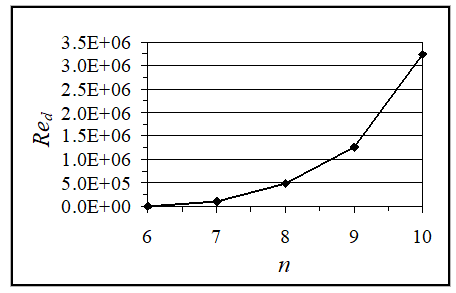
\includegraphics[width = 0.7 \textwidth]{../img/diagram85.png}
  \caption{Dependence of $n$ on Reynolds Number $Re_d$}
\end{figure}
\subsection{Friction factor}
The friction factor can be found empirically
\begin{itemize}
  \item \makebox[5cm]{Very approximately:\hfill} $2\sqrt{f} \approx \frac{1}{n}$
  \item \makebox[5cm]{\textit{Blasius} $\left(Re_d < 8 \times 10^4\right)$:\hfill} $f = 0.0791 Re_d^{-0.25}$
  \item \makebox[5cm]{\textit{Lees} $\left(Re_d < 4 \times 10^5\right)$:\hfill} $f=0.0019 + 0.153Re_d^{-0.35}$
\end{itemize}
Shear stress at wall:
\begin{equation}
  \tau_w = f \frac{1}{2} \rho \vec{U}^2
\end{equation}
Using \textit{Blasius's} friction factor and $n=7$ (i.e. $\vec{U} \approx 0.817U_{max}$)
\begin{equation}
  \tau_w = \left[ 0.0791\left(\frac{\rho \vec{U}d}{\mu}\right)^{-0.25} \right] \frac{1}{2}\rho \vec{U}^2 \rightarrow \tau_w = 0.0225 \rho U^2_{max} \left(\frac{\rho U_{max}a}{\mu}\right)^{-0.25}
\end{equation}
\section{Laminar flow in rough pipes}
To be truly smooth, the perturbations on the pipe wall surface would have to be small compared to the fluid molecules, i.e. no pipe is truly smooth in practice! \textit{Nikuradse} conducted experiments using pipes artificially roughened with sand grains. Roughness = $k$, Relative roughness = $\frac{k}{d}$. Alternative notation: $k_s$ = uniform bumps (sand grains), $k$ = more random (typical) distribution of size. Pipes of all $\frac{k}{d}$ behave in same manner for laminar flow, $f = f\left(Re_d\right)$:
\begin{align}
  f = \frac{16}{Re_d}
\end{align}
The critical $Re_d$ number for laminar to turbulent transition is independent of $\frac{k}{d}$. Once the flow is turbulent, the factor that determines flow behaviour is that sand grain height relative to the viscous sublayer thickness $\delta_L$.
\section{Turbulent flow}
\subsection{Universal laws}
Improved profiles by subdivision of flow: \textit{Universal Laws}. The universal laws are semi-empirical: The expressions have been derived theoretically but the constant have been found experimentally. Three layer concept:
\begin{figure}[H]
  \centering
  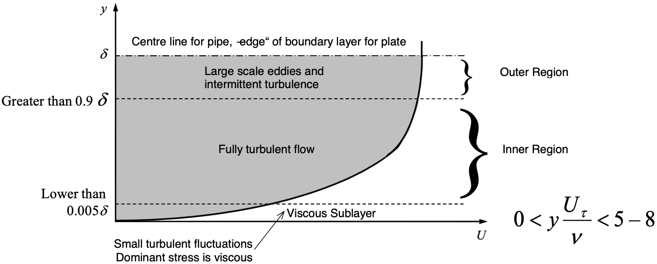
\includegraphics[width = 0.7 \textwidth]{../img/diagram87.png}
  \caption{}
\end{figure}
\begin{figure}[H]
  \centering
  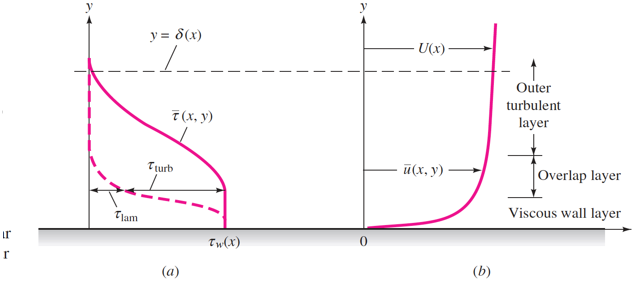
\includegraphics[width = 0.7 \textwidth]{../img/diagram88.png}
  \caption{}
\end{figure}
Friction velocity:
\begin{align}
  U_{\tau} = \sqrt{\frac{\tau_w}{\rho}}
\end{align}
Sublayer thickness:
\begin{align}
  \delta_L = \frac{5v}{U_{\tau}}
\end{align}
\section{Turbulent flow in rough pipes}
\begin{figure}[H]
  \centering
  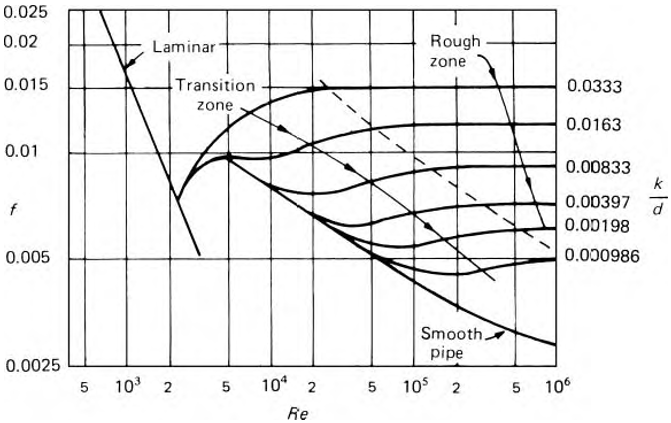
\includegraphics[width = 0.7 \textwidth]{../img/diagram86.png}
  \caption{}
\end{figure}
In the turbulent region there is a range of $Re_d$ over which a pipe of a given $\frac{k}{d}$ behaves as if it were a smooth pipe: the \textit{Hydraulically Smooth} pipe, $f = f\left(Re_d\right)$ only. The hydraulically smooth regime exists when $k < \delta_L$:
\begin{align}
  k < \delta_L \rightarrow \frac{k U_{\tau}}{v} < 5 \textrm{ or } k^+ < 5: \ \frac{1}{\sqrt{5}} = 4.0 \log \left(Re_d \sqrt{f}\right) - 0.4
\end{align}
Roughness elements immersed in viscous sublayer (no effect of roughness). At a particular $Re_d$ (which decreases as $\frac{k}{d}$ increases) the resistance law deviates from the smooth pipe law: the \textit{Smooth-Rough} transition $f = f\left(Re_d, \frac{k}{d}\right)$
\begin{align}
  5 < \frac{k U_{\tau}}{v} < 70 \textrm{ or } 5 < k^+ < 70
\end{align}
Roughness elements partly outside sublayer and provide additional resistance. Ultimately a region is reached where the friction factor is a function of relative roughness only: the \textit{Fully Rough} flow. $f = f\left(\frac{k}{d}\right)$ only.
\begin{align}
  \frac{kU_{\tau}}{v} > 70\textrm{ or } k^+ > 70: \ \frac{u}{U_\tau} = 5.75 \log \left(\frac{y}{k}\right) + 8.48 \ \frac{1}{\sqrt{f}} = 4/0\log \left(\frac{d}{2k}\right) +3.48
\end{align}
All roughness elements extend well beyond sublayer (no effect of $Re_d$)
\section{Flow in rough pipes}
The friction factor for rough-pipe flows is typically given by charts as a function of  the Reynolds number and pipe-wall roughness. These charts are based on experimental data and empirical correlations. Same "smooth pipe" line for all fluids, all pipe diameters and all flow velocities. Different behaviour for laminar and turbulent flows as expected, with ill-definition in transition region ($Re_{d, crit} = 2300$).
\begin{figure}[H]
  \centering
  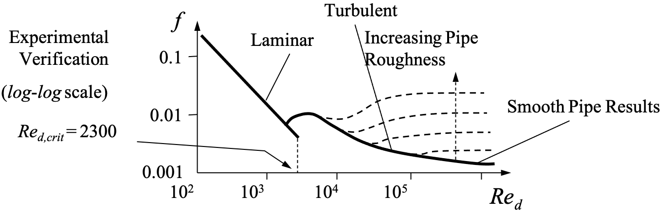
\includegraphics[width = 0.7 \textwidth]{../img/diagram89.png}
  \caption{}
\end{figure}
\section{the Moody chart for pipe flows}
\begin{figure}[H]
  \centering
  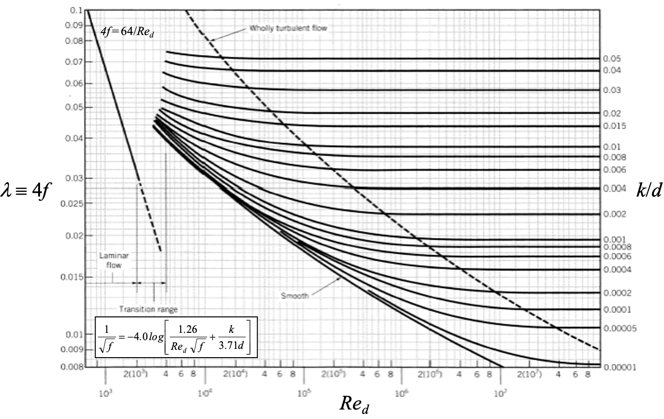
\includegraphics[width = 0.7 \textwidth]{../img/diagram90.png}
  \caption{Composite log-Law for Smooth and Rough pipes: Moody Chart ($\lambda = 4f$ on vertical axis)}
\end{figure}
\section{The Haaland approximation for pipe flows}
\begin{figure}[H]
  \centering
  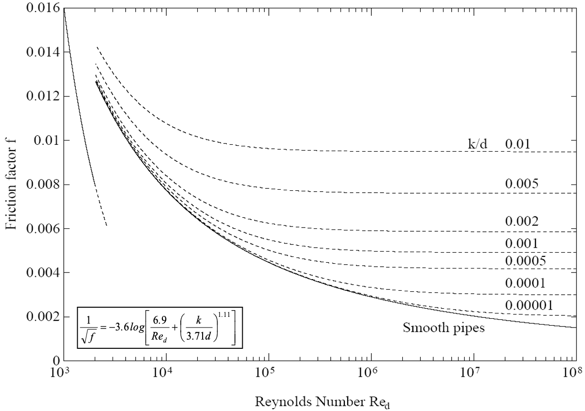
\includegraphics[width = 0.7 \textwidth]{../img/diagram91.png}
  \caption{Composite log-law for smooth and rough pipes: Haaland Formula chart ($f$ on vertical axis)}
\end{figure}
\end{document}